\documentclass[spanish,12pt,a4paper,titlepage]{report}
\usepackage[utf8]{inputenc}
\usepackage{graphicx}
\usepackage{subfig}
\usepackage{float}
\usepackage{wrapfig}
\usepackage{multirow}
\usepackage{caption}
\usepackage[spanish]{babel}
\usepackage[dvips]{hyperref}
\usepackage{amssymb}
\usepackage{listings}
\usepackage{epsfig}
\usepackage{amsmath}
\usepackage{array}
\usepackage[table]{xcolor}
\usepackage{multirow}
%\usepackage[Sonny]{fncychap}
\usepackage[Lenny]{fncychap}
%\usepackage[Glenn]{fncychap}
%\usepackage[Conny]{fncychap}
%\usepackage[Rejne]{fncychap}
%\usepackage[Bjarne]{fncychap}
%\usepackage[Bjornstrup]{fncychap}

%\usepackage{subfiles}
%\usepackage{framed}

\setlength{\topmargin}{-1.5cm}
\setlength{\textheight}{25cm}
\setlength{\oddsidemargin}{0.3cm} 
\setlength{\textwidth}{15cm}
\setlength{\columnsep}{0cm}

\begin{document}

\chapter{Test GPS}

\section{Objetivos}

Se realiza una serie de pruebas con el fin de identificar los errores correspondientes al dispositivo de posicionamiento global (\textbf{GPS}). Se realizan pruebas para determinar tanto el error absoluto de la medida, como el error diferencial. Se analizará el error en las direcciones de latitud, longitud y altura. A su vez se realizarán pruebas repetitivas de modo de poder analizar la consistencia temporal de las medidas otorgadas por el dispositivo GPS.

Si el error absoluto es muy grande, igual es posible obtener información útil utilizando medidas diferenciales. Se analizará el error relativo entre diferentes medidas del GPS. Resulta interesante caracterizar el comportamiento diferencial de las medidas del GPS ya que si es bueno, constituye una importante ventaja. Aunque el error absoluto sea grande, si el relativo es lo suficientemente chico se puede implementar alguna etapa de corrección inicial de modo de obtener datos georeferenciados muy precisos.\\

\section{Materiales}
\begin{itemize}
\item GPS
\item Brújula
\item Plomada
\item Metro
\end{itemize}

\section{Parte I: Error absoluto}
Tomar una medida de posición del GPS, en lo posible lugar de coordenadas conocidas. Contrastar los resultados obtenidos con las coordenadas conocidas. Ubicar las coordenadas en un mapa\footnote{\underline{Nota:} El mapa no debe ser de Google Earth ya que posee errores demasiado grandes. Usar mapas de la intendencia.}. Conseguir un mapa topográfico y obtener la altura respecto del nivel del mar de esa zona y contrastar con la altura obtenida del GPS. \\

Realizar este experimento en 3 lugares diferentes, 3 veces en cada lugar.

\newpage
\section{Parte II: Error relativo en latitud y longitud}

En esta prueba se trata de obtener el error del GPS en el plano paralelo a la tierra.

El experimento que se diseñó consiste en marcar un rectángulo sobre el suelo (pasto), utilizando 6 puntos, con la siguiente disposición:

\begin{quote}
\begin{quote}
\begin{quote}
\begin{verbatim}
<- <- Av Italia hacia el centro <- <-

4                5                6
x ---- ---- ---- x ---- ---- ---- x
|                                 |
|                                 |

|                                 |
|                                 |
x ---- ---- ---- x ---- ---- ---- x
1                2                3

-> -> Av Italia hacia el este -> ->
\end{verbatim}
\end{quote}
\end{quote}
\end{quote}

Todas las líneas punteadas son de 1m de largo, lo que resulta en un rectángulo de 1m por 2m.

Los pasos a seguir son los siguientes:

\begin{enumerate}
\item Construir un rectángulo como el mencionado sobre un superficie plana.
\item Medir, con un metro, las distancias entre todos los puntos.
\item Utilizar mínimos cuadrados para minimizar el error entre las distancias esperadas, y las experimentales. Esto puede llevar a trabajar con un polígono que \textbf{no} sea un rectángulo, pero el error será menor que el que resultaría de usar los valores teóricos.
\item Fijar la altura y la orientación del GPS, y tomar medidas en cada uno de los puntos \verb+[1,2,3,4,5,6]+.
\item Tomar un punto como origen, y comparar la figura que resulta de los datos provenientes del GPS con las medidas tomadas con el metro.
\end{enumerate}

Este experimento permitirá estimar, en un caso muy hipotético, la performance que se puede esperar del GPS. El caso real, montado en el quad, estará afectado por vibraciones e interferencia causada por la presencia de los motores y la electrónica.

De cualquiera forma, este experimento sirve para establecer que \textbf{no} se puede esperar del GPS.

En la figura \ref{fig:gps_setup.png} se observa el experimento. Se utilizó una escalera para tener el GPS a una altura fija, separado del piso. Al nivel del piso los rebotes degradan seriamente la performance del GPS. Las 4 patas de la escalera se utilizaron para alinear el punto que se deseaba medir.

\textbf{NOTA:} Se probaron distintas orientaciones. Cabe destacar que la posición absoluta de los puntos medidos con la escalera en distintas orientaciones darán distintos resultados, ya que el centro de las 4 patas no coincide con la posición del GPS, que estaba fijo a la parte más alta de la escalera. Esto implica que no tiene sentido comparar medidas correspondientes a distintas orientaciones, sino comparar los datos de cada orientación contra las medidas tomadas con el metro.

\begin{figure}[h!]
  \begin{center}
  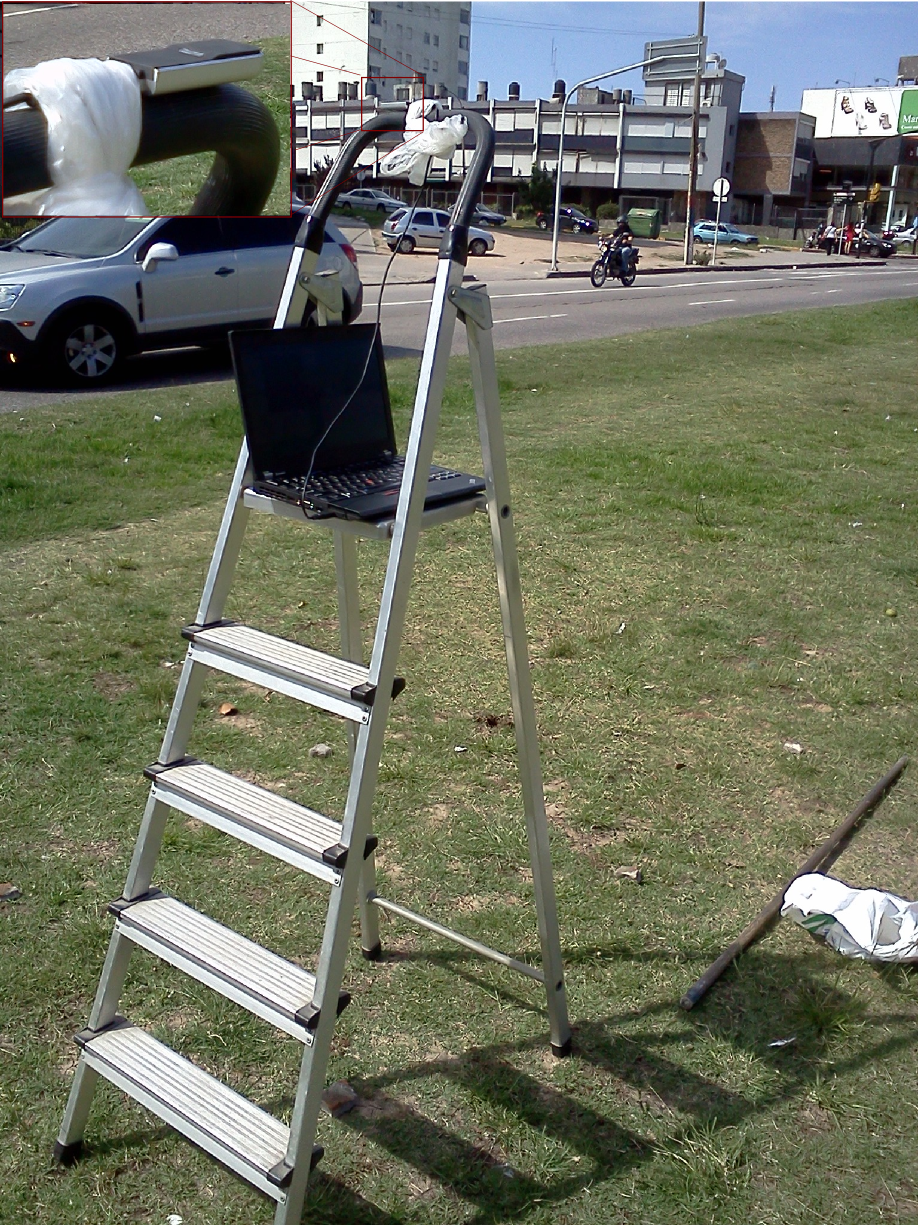
\includegraphics[width=.7\textwidth]{./img/gps_setup.png}
  \end{center}
  \caption{Experimento con el GPS.}
  \label{fig:gps_setup.png}
\end{figure}

\newpage

\subsection{Posibles fuentes de rebotes/interferencia}
\label{sec:posibles-fuentes-de-rebotes-interferencia}

Se buscó un lugar abierto, para evitar errores que puedan surgir por rebotes en paredes, edificios, etc. De cualquier forma, no se hizo el experimento en un lugar completamente abierto, ya que no se contaba con uno.

En las figuras \ref{fig:gps_interf.jpg} y \ref{fig:gps_interf1.jpg} se muestran posibles fuentes de rebotes/interferencia:

\begin{figure}[h!]
  \begin{center}
  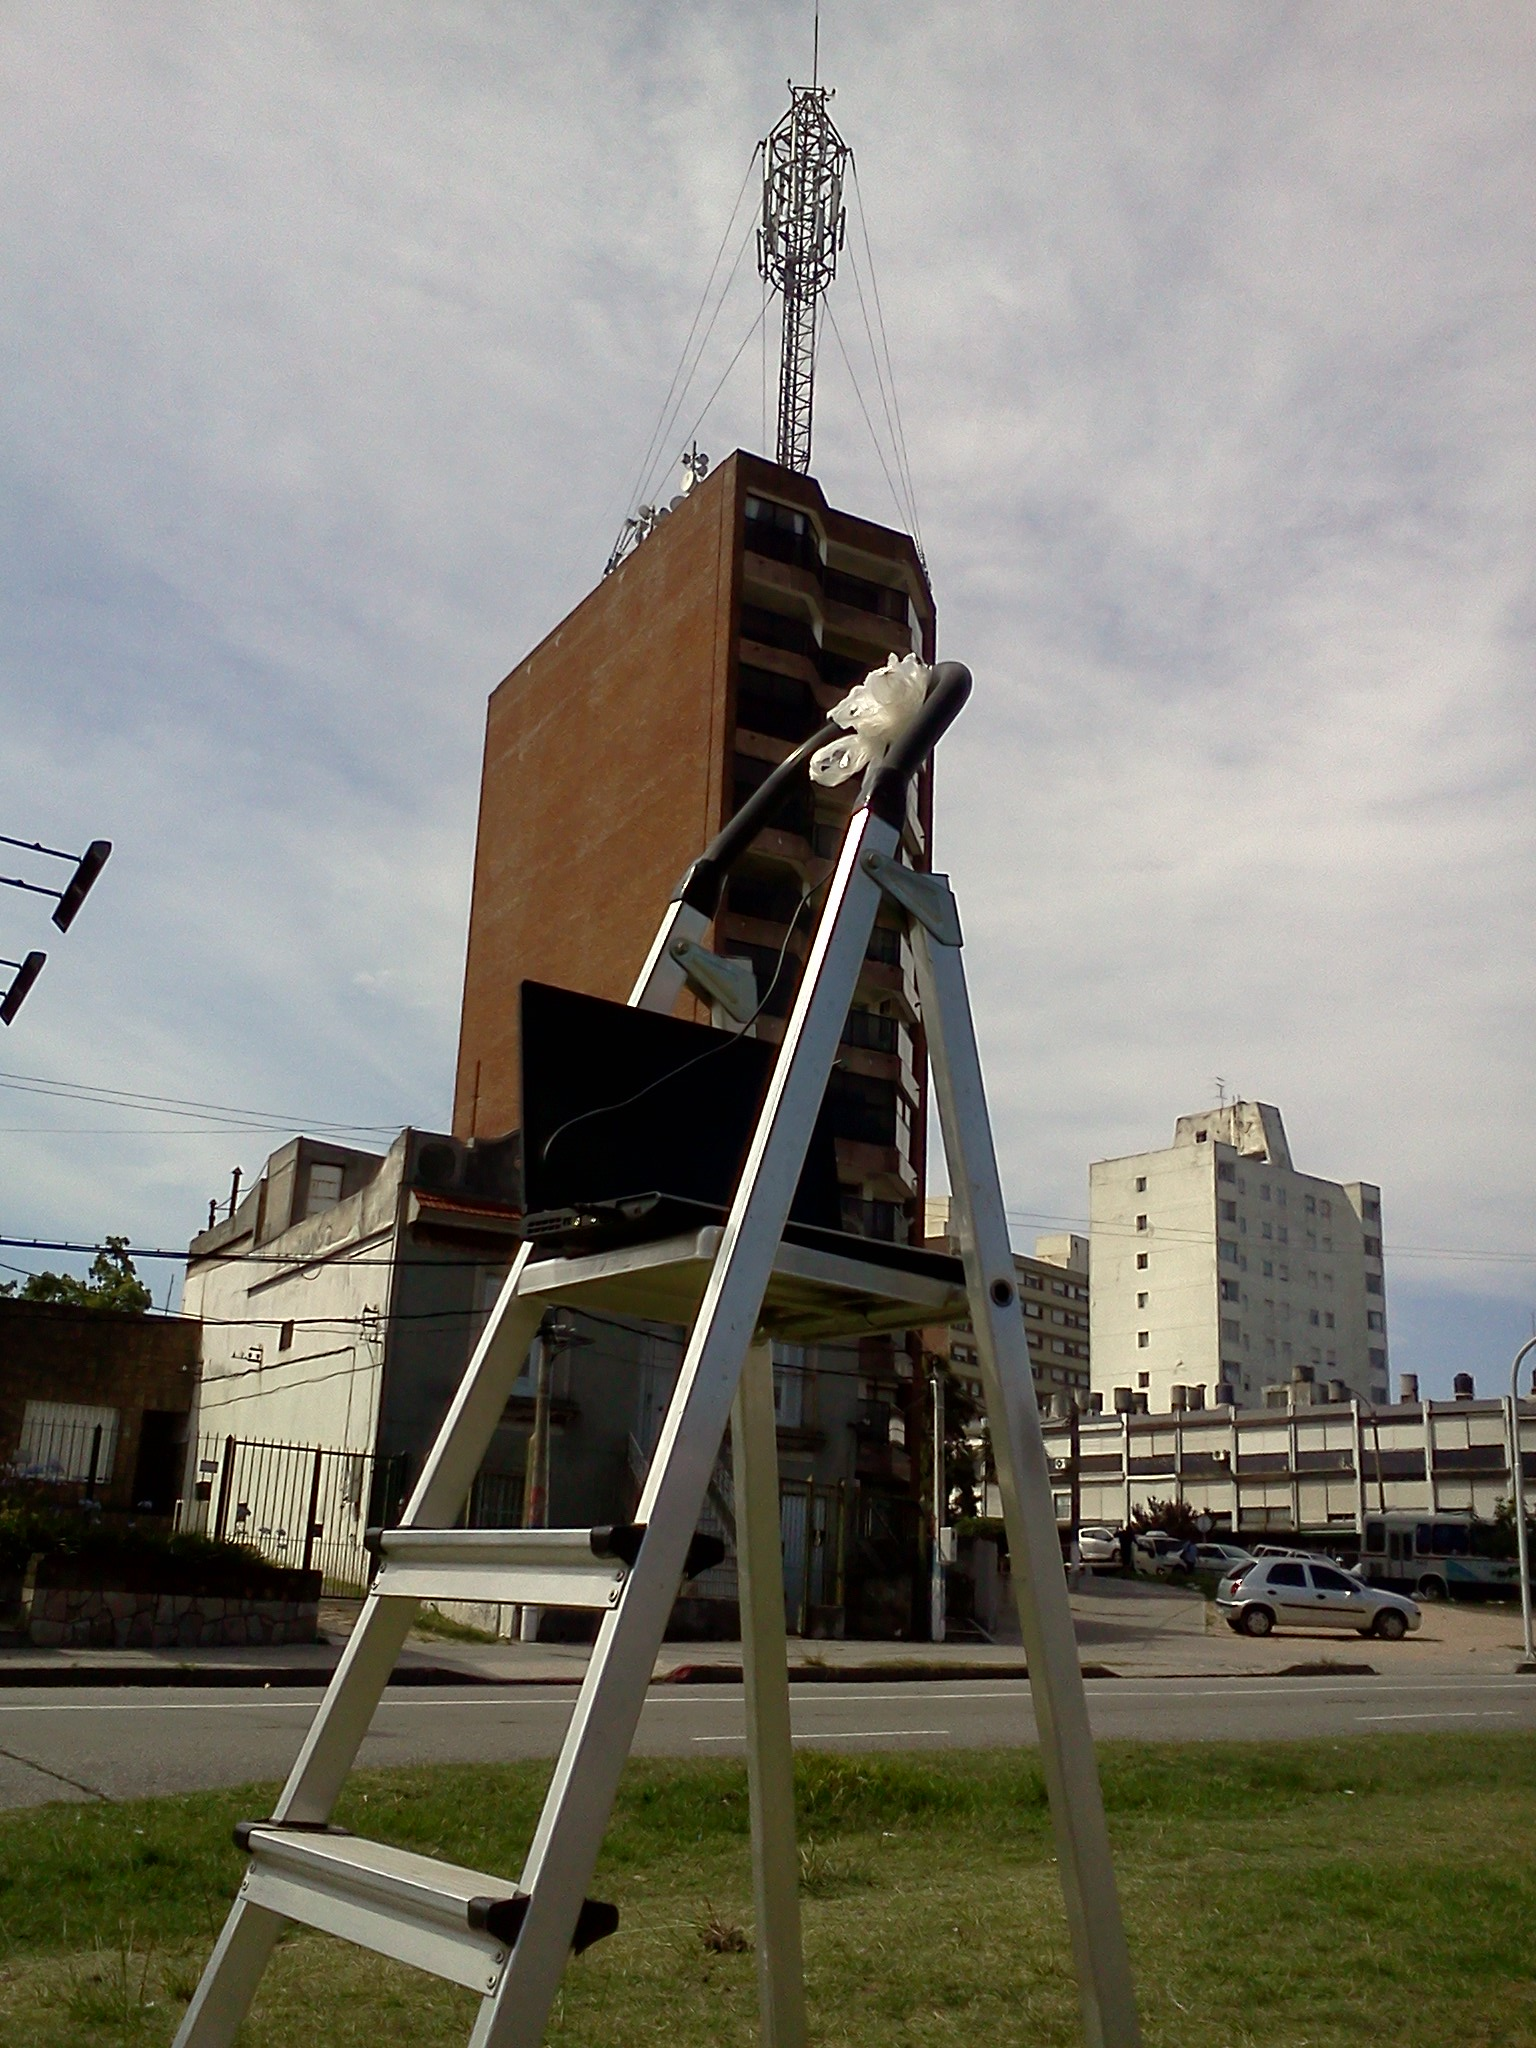
\includegraphics[width=.9\textwidth]{./img/gps_interf.jpg}
  \end{center}
  \caption{Rebotes/Interferencia: Edificio con antena.}
  \label{fig:gps_interf.jpg}
\end{figure}

\newpage
\begin{figure}[h!]
  \begin{center}
  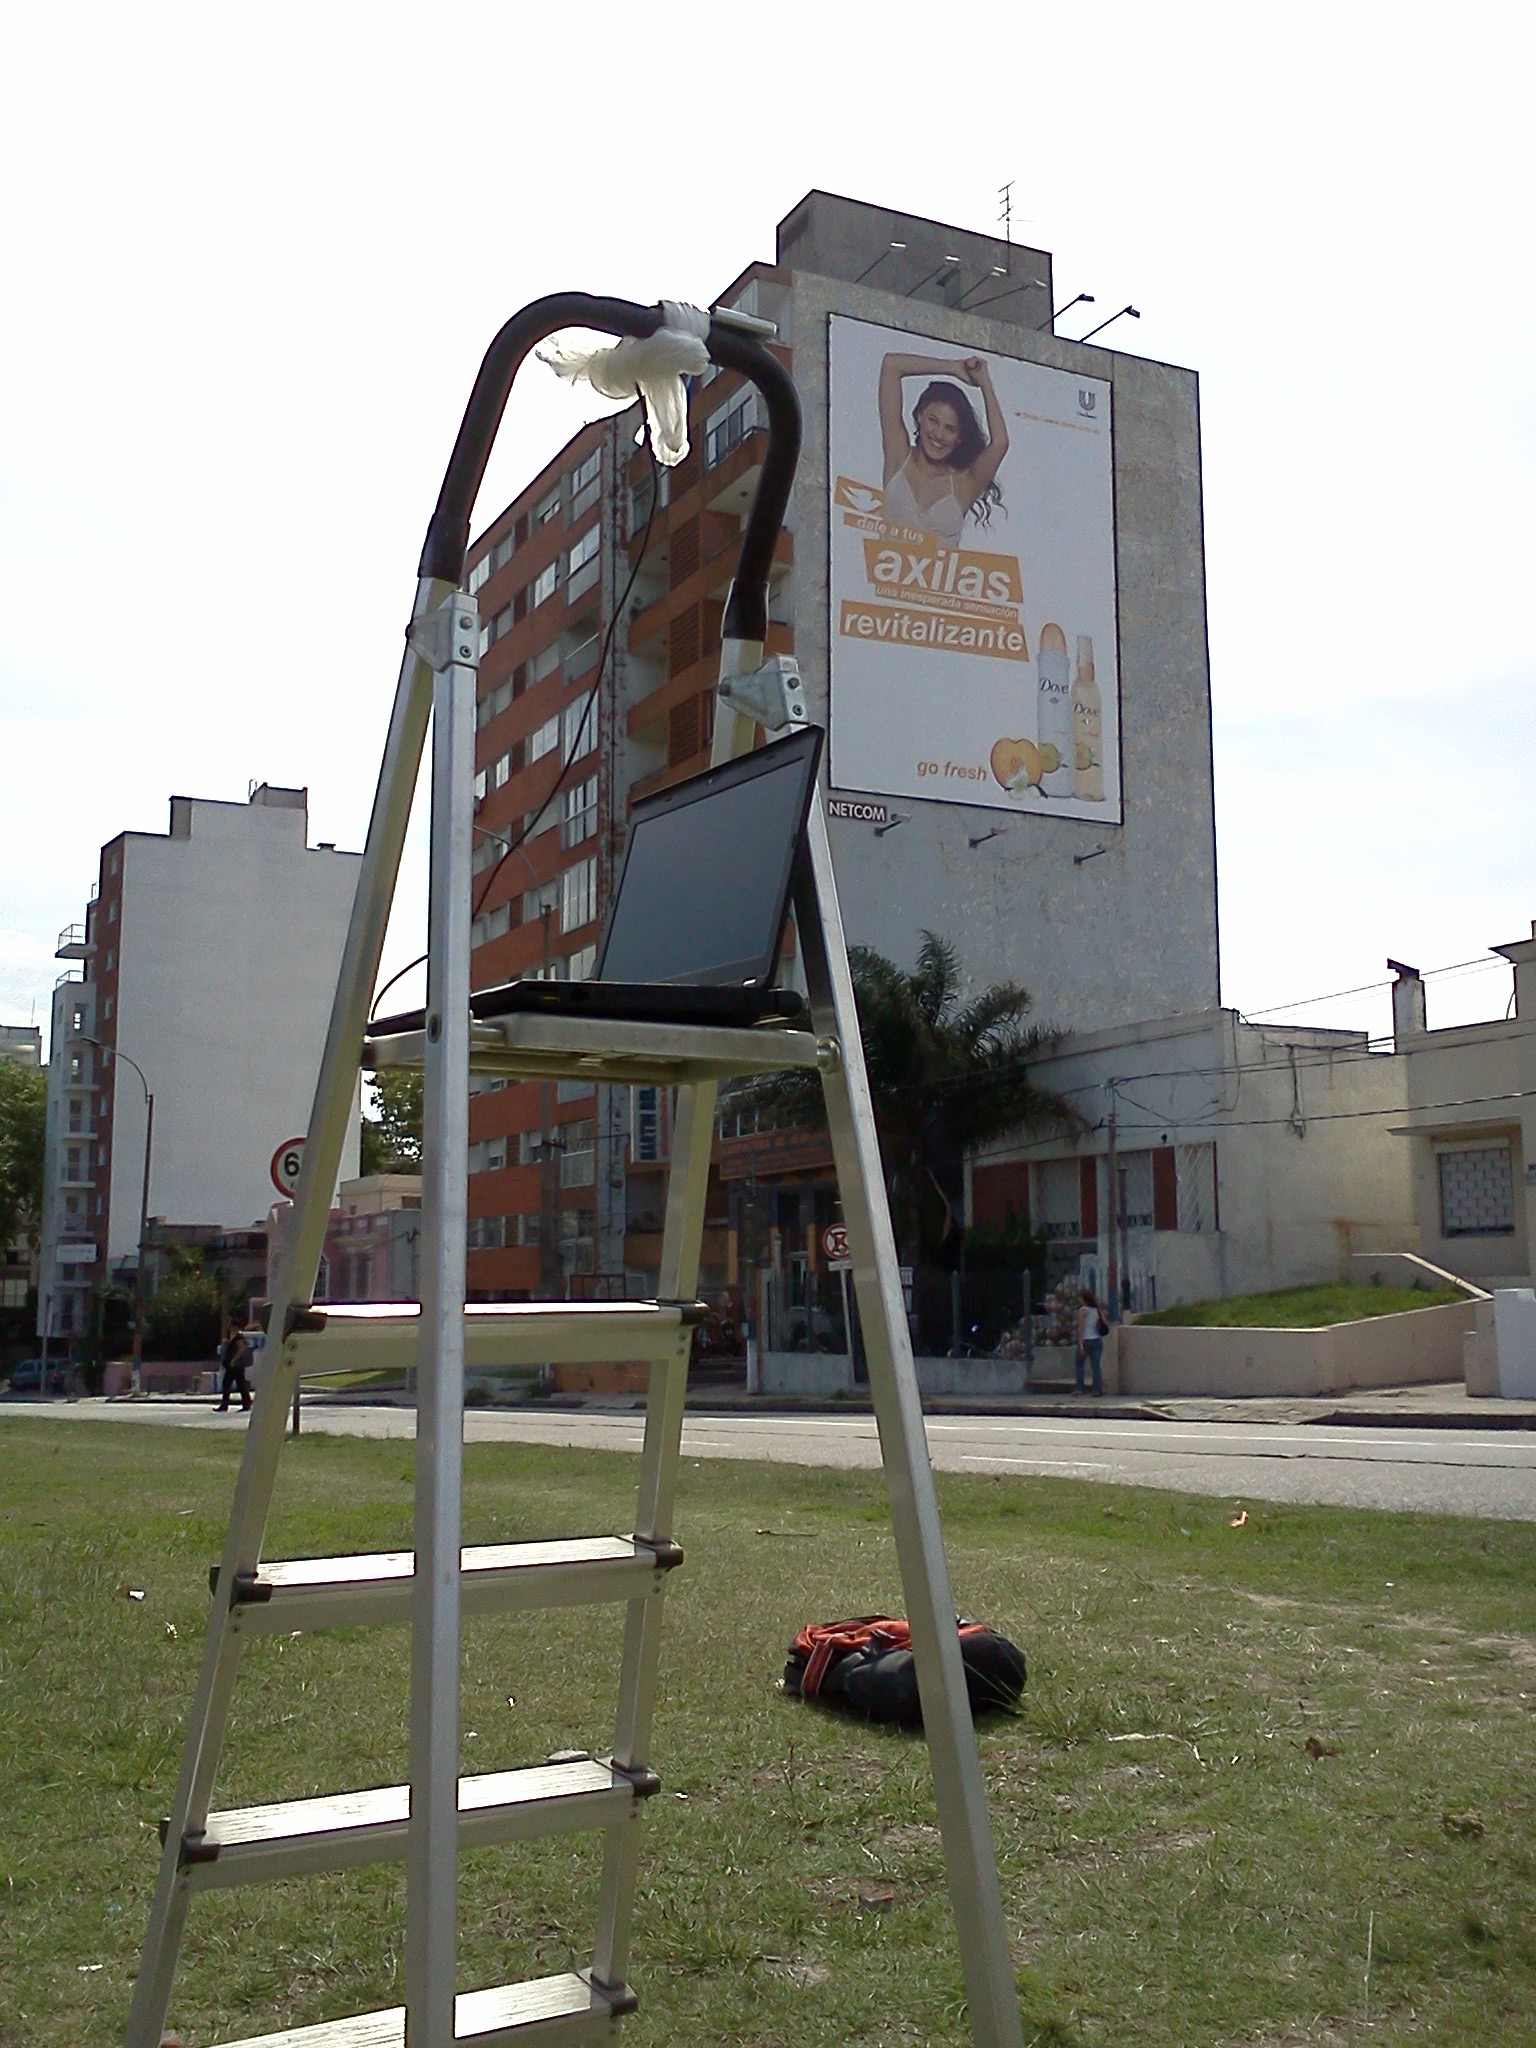
\includegraphics[width=.9\textwidth]{./img/gps_interf1.jpg}
  \end{center}
  \caption{Rebotes/Interferencia: Edificio.}
  \label{fig:gps_interf1.jpg}
\end{figure}

\newpage
\subsection{Estimación de la posición de un punto fijo}
\label{sec:estimacion-de-la-posicion-de-un-punto-fijo}

Antes de proceder con el experimento, se tomaron medidas de la ubicación de algunos de los vértices del polígono. Si el ruido asociado a esta medida supera 1m, entonces no vale la pena hacer el resto del experimento. No será posible estimar, de manera razonable, la posición de los vértices del polígono, ya que estos están distan, en algunos casos, solamente 1m entre sí.

Se tomaron medidas con el GPS en dos orientaciones. En las figuras \ref{fig:log_09_individual.png} y \ref{fig:log_10_individual.png} se observan los datos resultantes luego de aproximadamente 1 minuto con el GPS quieto. En todas las gráficas se muestran los datos luego de restar el promedio, o sea que se muestra el error respecto al valor promedio.

\subsubsection*{Punto 1}
\label{sec:punto-1}

\begin{figure}[h!]
  \hspace{-70pt}
  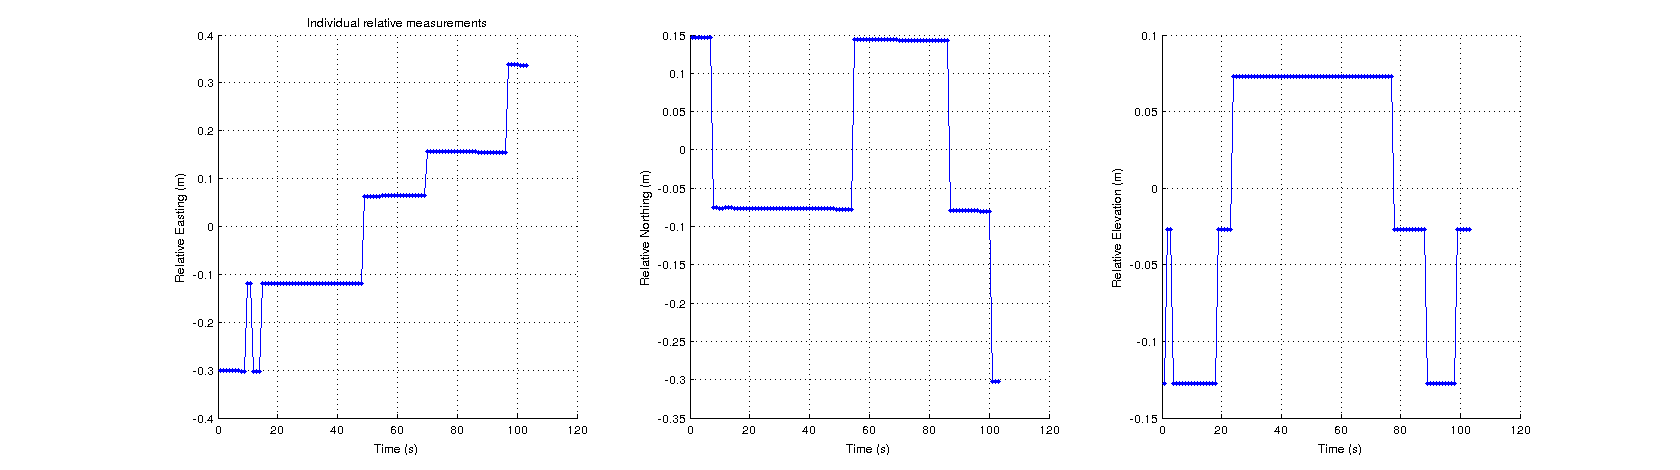
\includegraphics[width=1.3\textwidth]{./img/log_09_individual.png}
  \caption{GPS quieto en el punto 1, orientado [usb-led, 1-2].}
  \label{fig:log_09_individual.png}
\end{figure}

\begin{figure}[h!]
  \hspace{-70pt}
  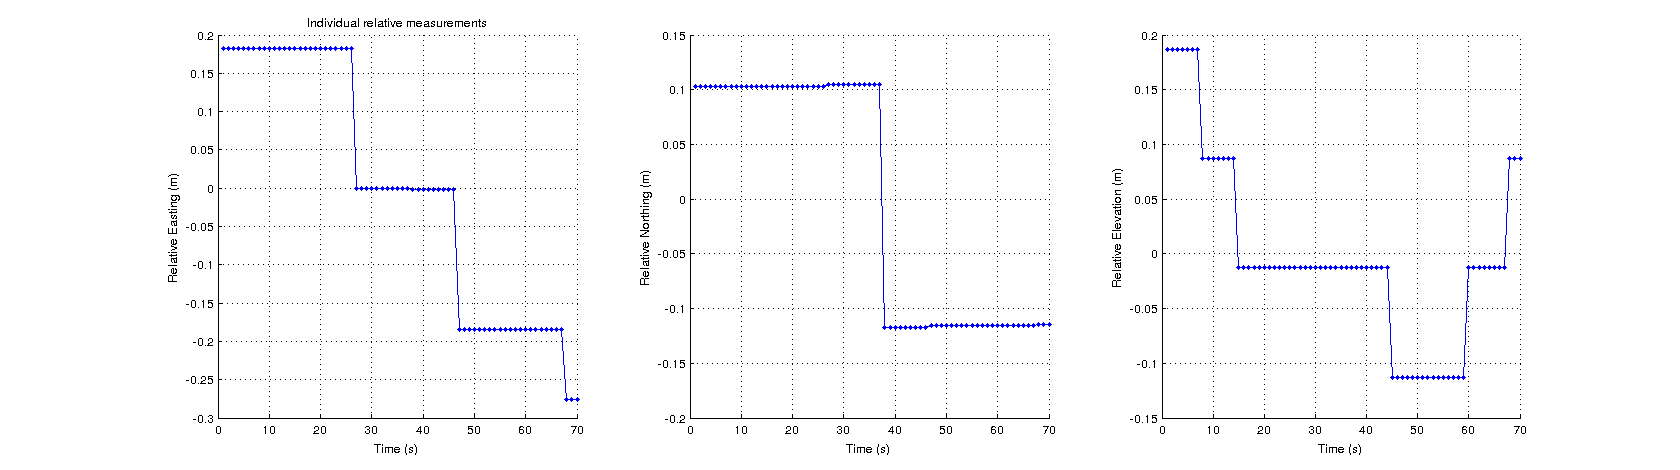
\includegraphics[width=1.3\textwidth]{./img/log_10_individual.png}
  \caption{GPS quieto en el punto 1, orientado [usb-led, 2-1].}
  \label{fig:log_10_individual.png}
\end{figure}

\newpage
\subsubsection*{Punto 4}
\label{sec:punto-4}

\begin{figure}[h!]
  \hspace{-70pt}
  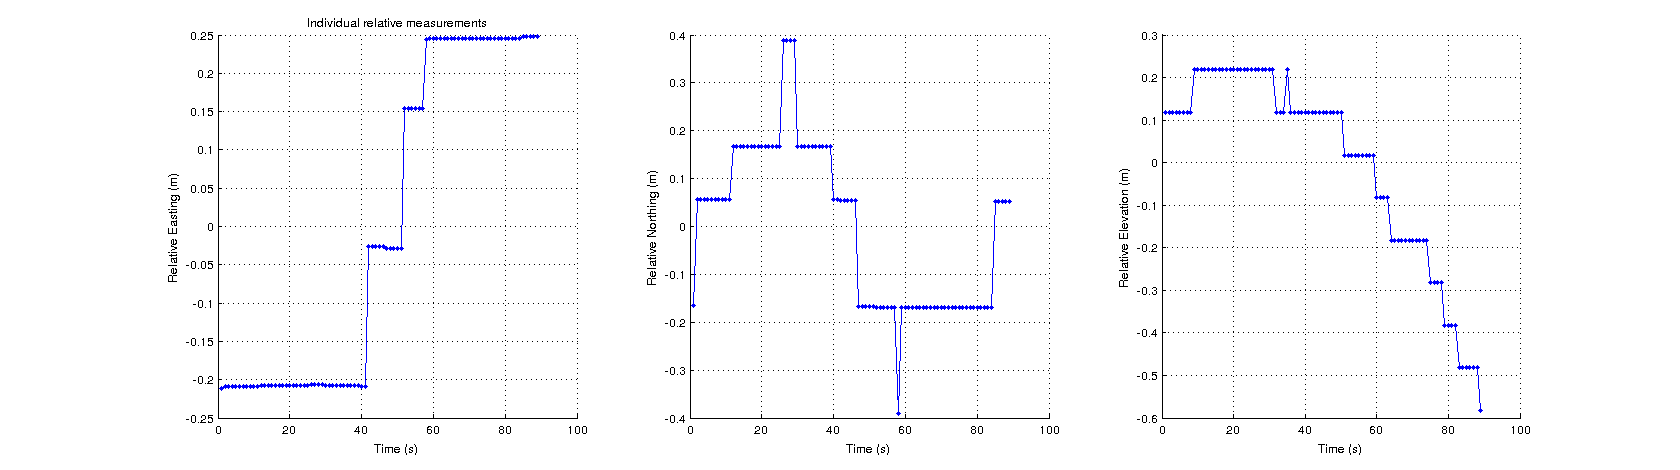
\includegraphics[width=1.3\textwidth]{./img/log_08_individual.png}
  \caption{GPS quieto en el punto 4, orientado [usb-led, 1-2].}
  \label{fig:log_08_individual.png}
\end{figure}

\begin{figure}[h!]
  \hspace{-70pt}
  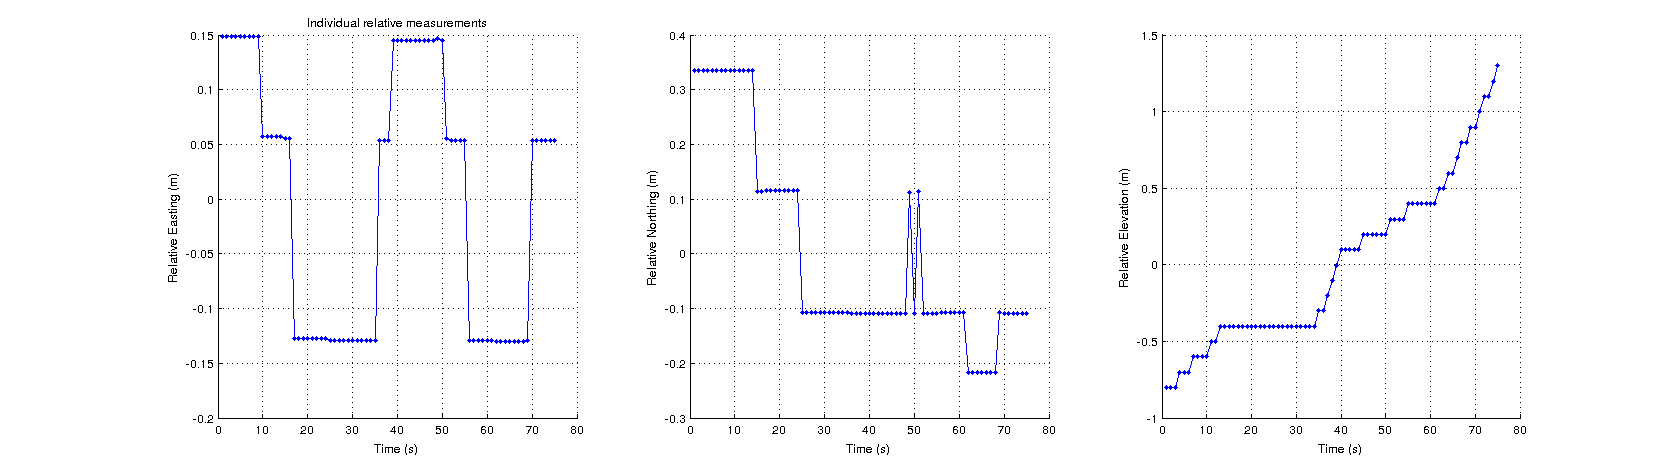
\includegraphics[width=1.3\textwidth]{./img/log_07_individual.png}
  \caption{GPS quieto en el punto 4, orientado [usb-led, 2-1].}
  \label{fig:log_07_individual.png}
\end{figure}

\subsubsection*{Punto 6}
\label{sec:punto-6}

\begin{figure}[h!]
  \hspace{-70pt}
  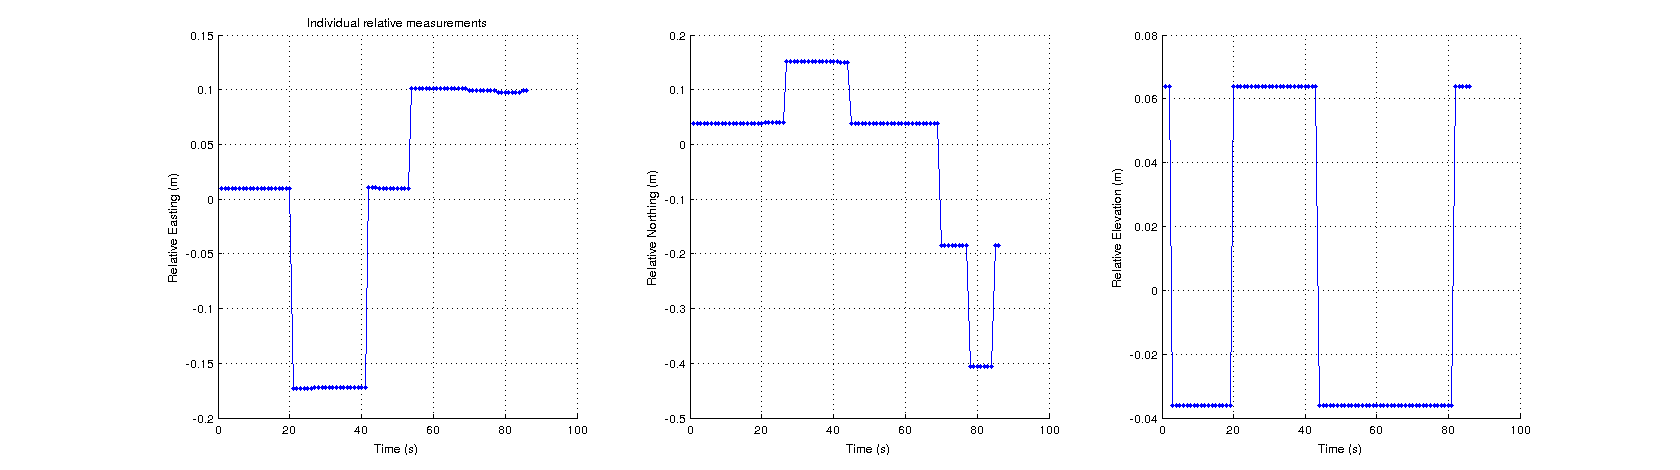
\includegraphics[width=1.3\textwidth]{./img/log_06_individual.png}
  \caption{GPS quieto en el punto 6, orientado [usb-led, 1-2].}
  \label{fig:log_06_individual.png}
\end{figure}

\newpage

\begin{figure}[h!]
  \hspace{-70pt}
  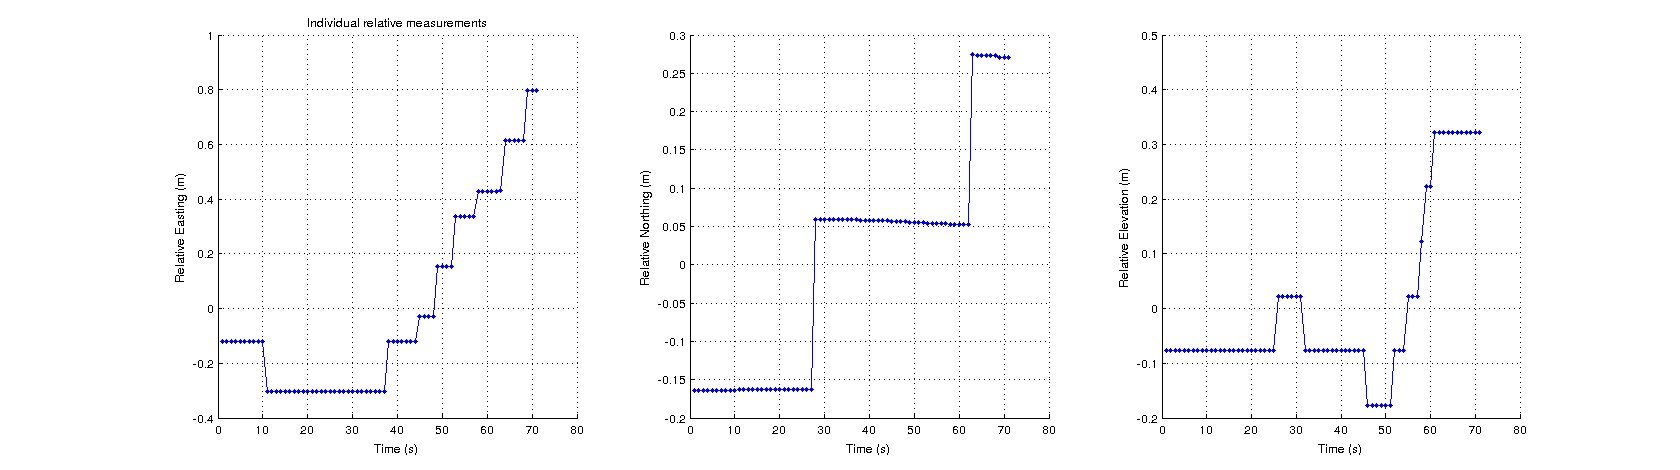
\includegraphics[width=1.3\textwidth]{./img/log_05_individual.png}
  \caption{GPS quieto en el punto 6, orientado [usb-led, 2-1].}
  \label{fig:log_05_individual.png}
\end{figure}

\subsubsection{Punto fijo: Conclusiones}
\label{sec:punto-fijo-conclusiones}

En varios casos se observaron errores del orden del metro, pero en otros el error fue menor a medio metro. No se esperan buenos resultados a priori, la precisión del GPS no parece adecuada para este experimento.

De cualquier forma se procedió con el experimento, tomando datos con el GPS en 4 orientaciones por si la precisión resulta muy sensible a la posición de la antena.

\newpage
\subsection{Polígono}
\label{sec:poligono}

Como era de esperarse, la precisión del GPS no resultó adecuada para este experimento. En las figuras \ref{fig:polygon_1.png} y \ref{fig:polygon_2.png} se observa lo que debería ser un rectángulo.

\begin{figure}[h!]
  \begin{center}
  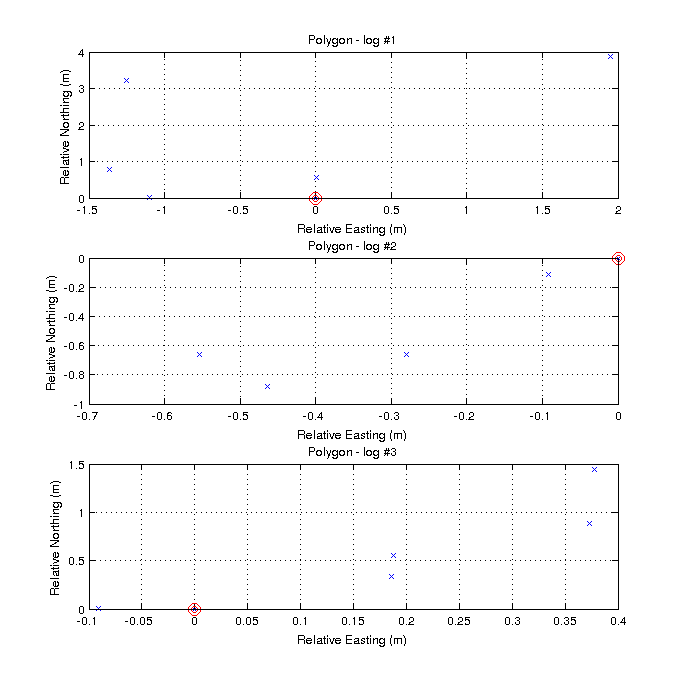
\includegraphics[width=1\textwidth]{./img/polygon_1.png}
  \end{center}
  \caption{Primeros 3 intentos de estimar el polígono.}
  \label{fig:polygon_1.png}
\end{figure}

\newpage
\begin{figure}[h!]
  \begin{center}
  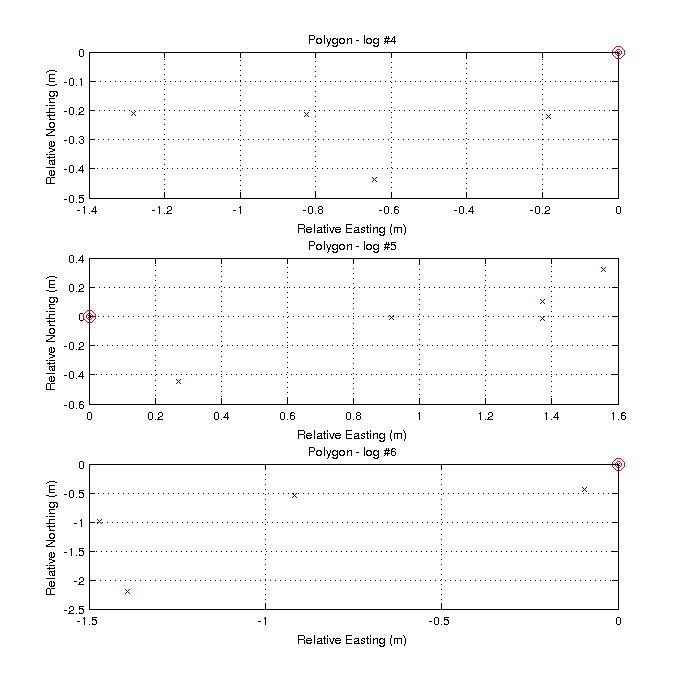
\includegraphics[width=1\textwidth]{./img/polygon_2.png}
  \end{center}
  \caption{Segundos 3 intentos de estimar el polígono.}
  \label{fig:polygon_2.png}
\end{figure}

En la tabla \ref{tab:polygon-sat} se muestran la cantidad de satélites utilizados cuando se obtuvieron los datos de las figuras \ref{fig:polygon_1.png} y \ref{fig:polygon_2.png}.

\begin{table}[H]
\begin{center}
\begin{tabular}{|l||c|c|c|c|c|c|}
\hline
\textbf{Log 1} & 8 & 8 & 8 & 7 & 8 & 8 \\
\hline
\textbf{Log 2} & 9 & 9 & 9 & 9 & 9 & 9 \\
\hline
\textbf{Log 3} & 9 & 9 & 9 & 9 & 9 & 9 \\
\hline
\textbf{Log 4} & 10 & 10 & 10 & 10 & 10 & 10 \\
\hline
\textbf{Log 5} & 10 & 10 & 10 & 10 & 10 & 10 \\
\hline
\textbf{Log 6} & 10 & 10 & 10 & 10 & 10 & 10\\
\hline
\end{tabular} 
\caption{Satelites disponibles al tomar los datos de las figuras \ref{fig:polygon_1.png} y \ref{fig:polygon_2.png}.}
\label{tab:polygon-sat}
\end{center}
\end{table}

\newpage
\subsubsection*{Errores}
\label{sec:errores}

Las especificaciones del GPS garantizan un error menor a 3m. La distancia de cada punto al punto 1 sirve para mostrar que el GPS cumple con las especificaciones. 

\begin{verbatim}
>> sqrt(easting.^2 + northing.^2)

ans =

  Columns 1 through 2

                         0                         0
         0.554512260087323         0.143700779969825
          4.33004706557553         0.143700779969825
          1.57529195895029         0.862204669928841
          3.46128113366155         0.997959241296461
          1.09657686103998           0.7196747757109

  Columns 3 through 4

                         0                         0
        0.0913813877153522         0.287401564952104
          0.37960034205882         0.287401564952104
         0.583854507635003         0.778438910449184
         0.959566360784181         0.851817377628425
          1.48734655792341          1.29842494542402

  Columns 5 through 6

                         0                         0
         0.521483162980721         0.452924086277894
          1.37072089636507         0.452924086277894
          1.58871200295859          1.06889681896435
         0.913813929586754          1.77030855041003
          1.37520004160367          2.60741605799409
\end{verbatim}

\subsection{Conclusión}
\label{sec:error-lat-lon-conclusion}

El GPS funciona como era de esperarse, con un error menor a 3m. Para estimar la posición del quad con más precisión, va a ser necesario recurrir a sensores adicionales, o a algún tipo de manipulación de los datos del GPS.

Este experimento se realizó libre de ruido. El quad agregará vibraciones, interferencia electromagnética, y sera mucho menos estable que el GPS aferrado a una escalera. El error en las medidas de este experimento fue, en general, significativamente menor a 3m, pero una vez montado en el quad, es probable que el error en la información proveniente del GPS sea cercana a los 3m, por culpa de los factores mencionados.

%
%\begin{enumerate} 
%	\item Seleccionar 4 puntos distintos y asegurarse que estén a la misma altura. En lo posible formando un rectángulo siguiendo las direcciones de latitud y longitud, según lo indique la brújula.
%	\item Tomar las medidas con un metro lo más cuidadosamente posible entre los 4 vértices, y los ángulos que forman las parejas de caras consecutivas.
%	\item Obtener el dato del GPS de los 4 vértices.
%	\item Obtener la diferencia entre medidas
%	\item Convertir datos a unidades del sistema métrico.
%	\item Reproducir el paralelepípedo en un esquema según los datos obtenidos del GPS.
%	\item Contrastar medidas y ángulos reales con los obtenidos del GPS.
%\end{enumerate} 
%

\section{Error en altura}
\label{sec:error-en-altura}

Para determinar el error la información sobre la altura que provee el GPS, se diseñó un experimento, que consiste en tomar medidas en una perpendicular a la esfera terrestre, a 4 alturas diferentes: 0m, 1m, 2m y 3m respecto al suelo.

En la primera etapa del experimento, se mantuvo el GPS quieto en cada uno de los niveles, y se tomaron muestras durante aproximadamente 60 segundos. El objetivo de esta etapa era verificar si era viable el experimento.

\subsection{Punto fijo}
\label{sec:altura-punto-fijo}

Para este experimento se colocó una escalera en el medio del estacionamiento de atrás de la Facultad de Ingeniería, se ató un piolín con marcas cada 1 metro, y una plomada en la punta para mantenerlo tenso y vertical.

\begin{figure}[h!]
  \begin{center}
  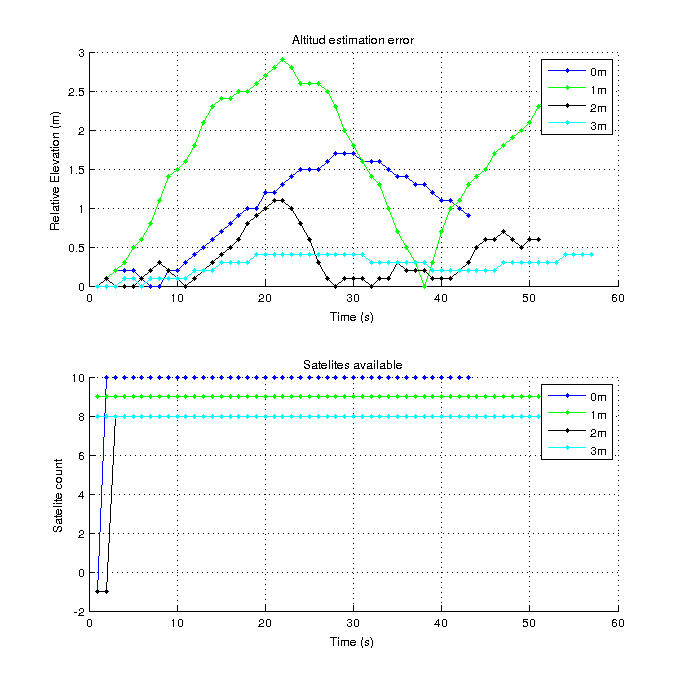
\includegraphics[width=.7\textwidth]{./img/altura_punto_fijo_fing.png}
  \end{center}
  \caption{Variación de la altura determinada por el GPS a distintas alturas.}
  \label{fig:altura_punto_fijo_fing.png}
\end{figure}

En la figura \ref{fig:altura_punto_fijo_fing.png} se observan los resultados del experimento. Es de esperarse que el error sea mayor al estar apoyado sobre el suelo, ya que los rebotes pueden deteriorar el sistema. El error a 1m de altura es mayor al que se obtuvo con el GPS en el suelo, una posible explicación para esto sería que el GPS estaba muy cerca de la escalera metálica, lo cual podría introducir una cantidad significativa de rebotes.

Los resultados de este experimento llevan a pensar que el GPS da información estable si y solo si se encuentra a al menos 2m del suelo. No se cuenta con suficiente información como para afirmar esto con certeza, por lo que se optó por tomar más datos, teniendo especial cuidado con el tema de los rebotes.

\subsection{Punto fijo - Estabilidad y rebotes}
\label{sec:altura-punto-fijo-estabilidad}

Para analizar el efecto de los rebotes sobre la estabilidad de la información proveniente del GPS, se tomaron varias series de datos con el GPS quieto, sobre el marco de una ventana, y luego asomado 1 metro hacia afuera (y arriba) de la ventana, donde el efecto de los rebotes debería ser menor.

En la figura \ref{fig:gps_gabi3.jpg} se observa la configuración del GPS al tomar los datos apoyado sobre el marco de la ventana, y en la figura \ref{fig:gps_gabi1.jpg} se observa el atril utilizado para alejar al GPS de la superficie.

\begin{figure}[h!]
  \begin{center}
\subfloat[GPS expuesto a rebotes sobre la superficie en la que se apoya.]{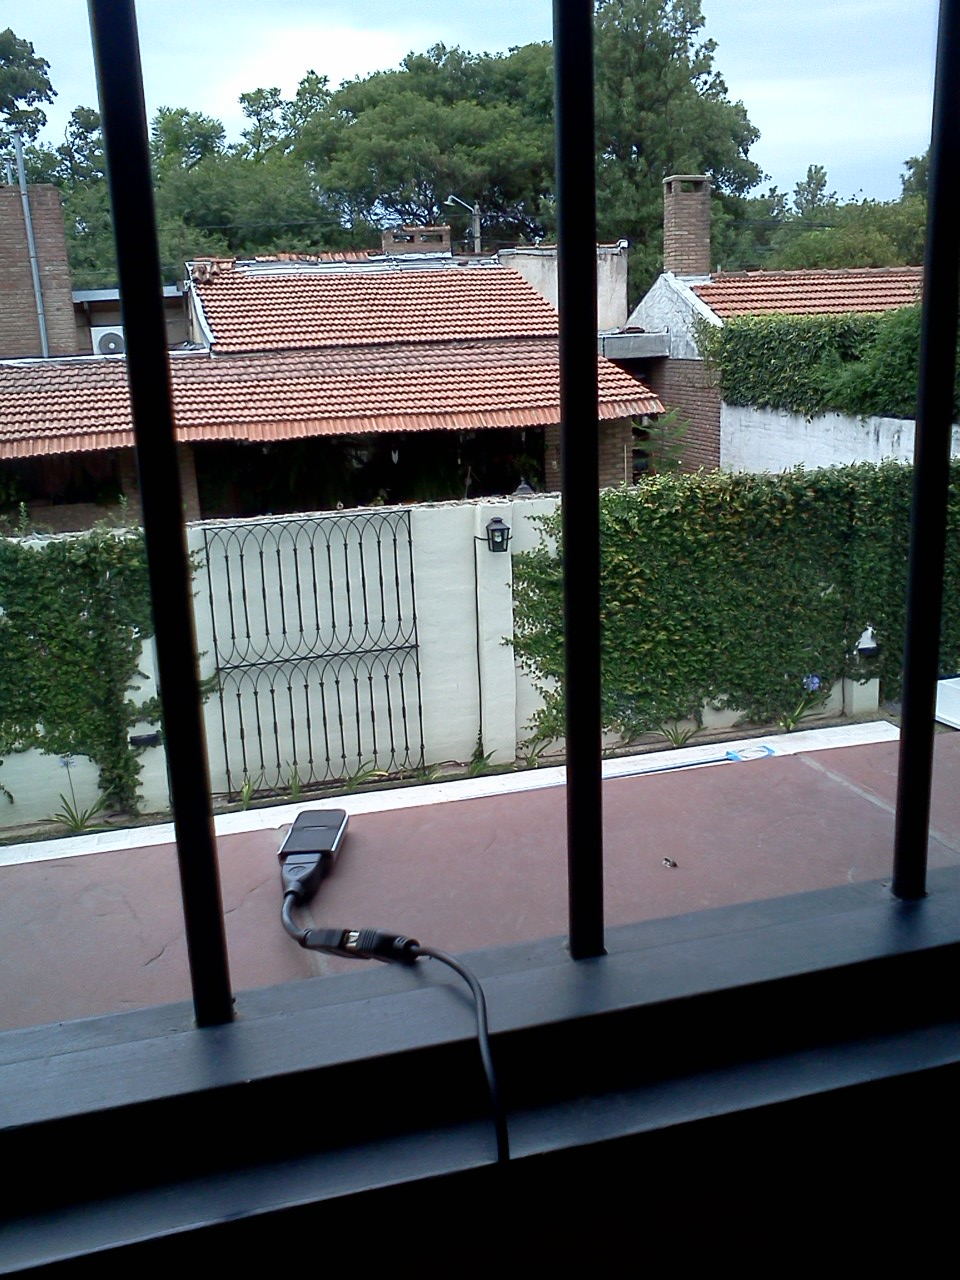
\includegraphics[width=.3\textwidth]{./img/gps_gabi3.jpg}\label{fig:gps_gabi1.jpg}}
\hspace{50pt}
\subfloat[GPS alejado de superficies.]{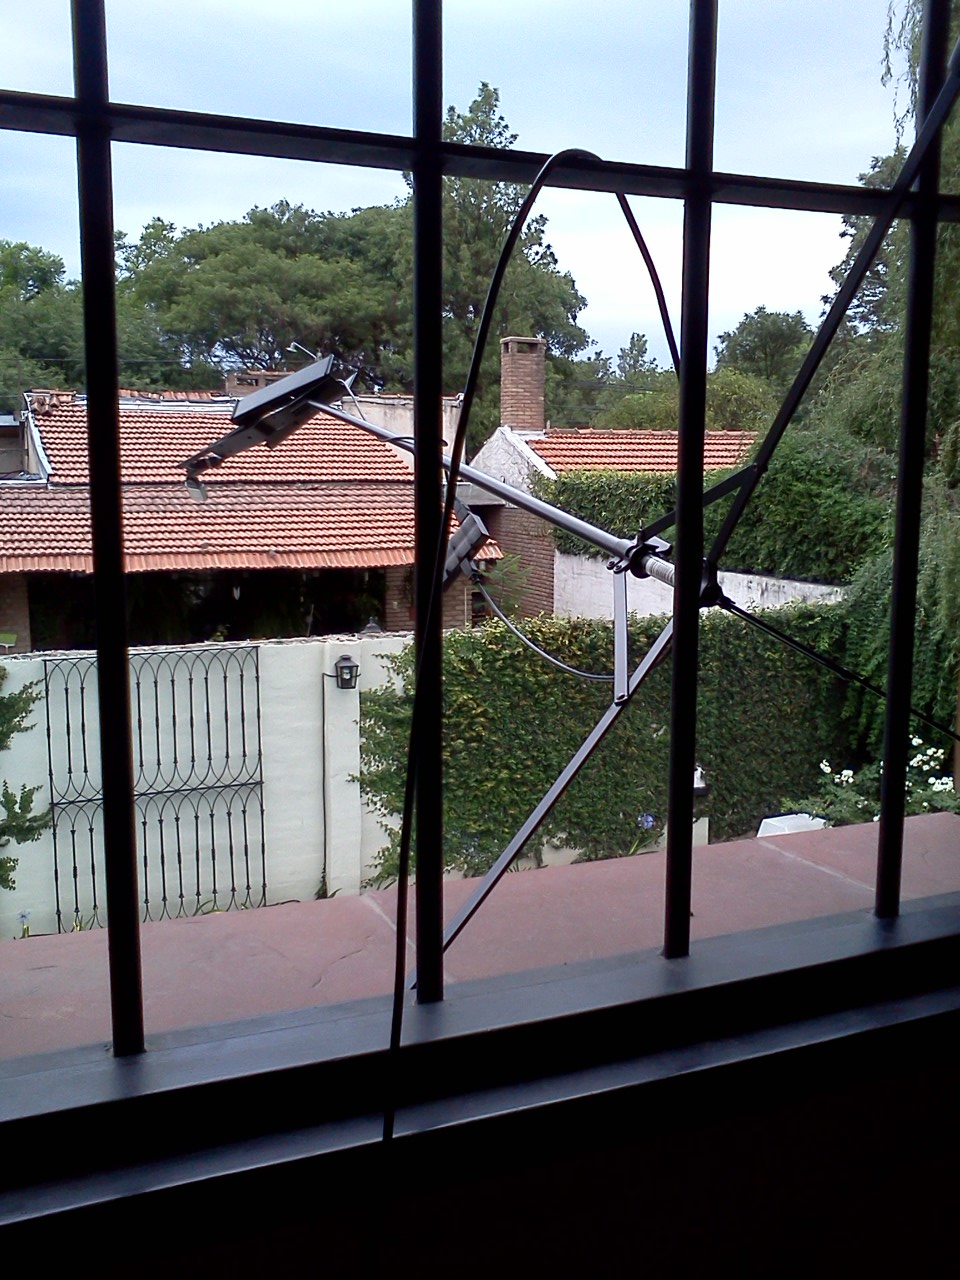
\includegraphics[width=.3\textwidth]{./img/gps_gabi1.jpg}\label{fig:gps_gabi3.jpg}}
  \end{center}
\end{figure}

Los resultados del experimento apoyado sobre el marco y asomado con el atril se observan en las figuras \ref{fig:gps_ventana.png} y \ref{fig:gps_atril.png} respectivamente.

\begin{figure}[h!]
  \begin{center}
  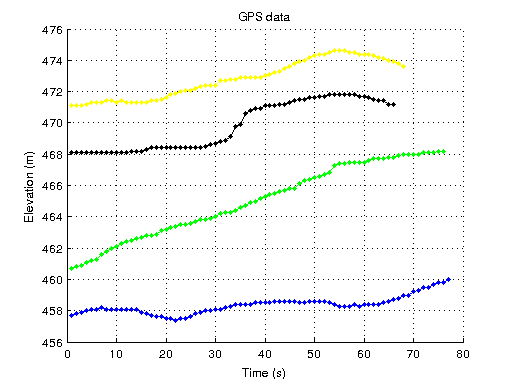
\includegraphics[width=.75\textwidth]{./img/gps_ventana.png}
  \caption{GPS apoyado sobre superficie.}
  \label{fig:gps_ventana.png}
\end{center}
\end{figure}

\newpage
\begin{figure}[h!]
\begin{center}
  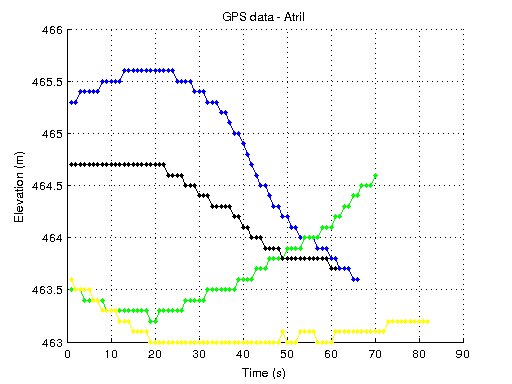
\includegraphics[width=.75\textwidth]{./img/gps_atril.png}
  \caption{GPS alejado de superficies.}
  \label{fig:gps_atril.png}
\end{center}
\end{figure}

\subsection{Conclusión}
\label{sec:error-en-altura-conclusion}

Los resultados concuerdan con lo esperado, la inestabilidad en la lectura del GPS disminuye al reducir las fuentes de rebotes.

Las lecturas del GPS no tiene suficiente precisión como para ser utilizadas de manera exclusiva para determinar la altura del quad. En los mejores casos hay un error de $0.5-1$m, y en los peores casos hay errores de hasta 15m. Con una buena geometría y a varios metros del piso, el error es tolerable, pero no sirve para programar el aterrizaje/despegue, ni el vuelo a baja altura.

Aún no se ha determinado si la mayor causa del deterioro de la performance del GPS fueron los rebotes y/o la mala geometría. La mala geometría resulta de tener solamente la mitad del cielo visible, ya que la pared de la casa bloquea el resto. Al asomar el GPS hacia afuera, se lo aleja de los rebotes, y también se incrementa la cantidad de cielo visible, por lo que es dificil separar cual de los cambios es el responsable de los cambios en los resultados.

Se concluye que es necesario utilizar otra fuente de información, como por ejemplo un sensor de presión, para estimar la altura del quad.

%\newpage

%\section{GPS con corrección diferencial}
%\label{sec:gps-diff}
%
%Para evaluar la performance del GPS en espacios más grandes, se relevó un polígono, tomando datos con el GPS a evaluar, junto con otro GPS que cuenta con correción diferencial, y es de mejor calidad.
%
%En la figura \ref se observa el camino recorrido, y los puntos de interés.
%
%\section{Parte III: Consistencia}
%
%Esta prueba se basa en la repetitividad de una misma prueba para analizar las diferencias entre los datos obtenidos por GPS en diferentes ocasiones.\\
%
%Se tomarán las medidas de los 4 puntos seleccionados en la parte anterior un total de 10 veces cada punto. Se analizarán los resultados obtenidos para caracterizar la consistencia del dispositivo GPS. Graficar las medidas obtenidas en latitud, longitud y altura para cada punto por separado. Hallar el error máximo de las medidas en un mismo punto.

%\section{Desarrollo}
%\subsection{Parte I: Error absoluto}
%
%\begin{table}[H]
%\begin{center}
%\begin{tabular}{|p{40pt}|p{110pt}|p{110pt}|p{110pt}|} 
%\hline
%  \cellcolor[gray]{0.8} \textbf{Medida} 
%& \cellcolor[gray]{0.8} \textbf{Posición 1} 
%& \cellcolor[gray]{0.8} \textbf{Posición 2} 
%& \cellcolor[gray]{0.8} \textbf{Posición 3} \\ \hline \hline
%\multicolumn{1}{|p{40pt}|}{\cellcolor[gray]{0.8}\textbf{1}} & \hspace{50pt}/ & \hspace{50pt}/ & \hspace{50pt}/ \\ \hline 
%\multicolumn{1}{|p{40pt}|}{\cellcolor[gray]{0.8}\textbf{2}} & \hspace{50pt}/& \hspace{50pt}/& \hspace{50pt}/ \\ \hline 
%\multicolumn{1}{|p{40pt}|}{\cellcolor[gray]{0.8}\textbf{3}} & \hspace{50pt}/& \hspace{50pt}/& \hspace{50pt}/ \\ \hline 
%\end{tabular} 
%\caption{Medidas GPS}
%\label{tab:I-medidas}
%\end{center}
%\end{table}
%
%\newpage
%\subsection{Parte II: Error relativo}
%
%\begin{table}[H]
%\begin{center}
%\begin{tabular}{|p{100pt}|p{100pt}|p{100pt}|p{100pt}|} \hline
%\cellcolor[gray]{0.8} \textbf{Punto 1} & \cellcolor[gray]{0.8} \textbf{Punto 2} & \cellcolor[gray]{0.8} \textbf{Punto 3} & \cellcolor[gray]{0.8} \textbf{Punto 4} \\ \hline \hline
%\hspace{50pt}/ & \hspace{50pt}/ & \hspace{50pt}/ & \hspace{50pt}/ \\ \hline 
%\end{tabular} 
%\caption{Medidas GPS}
%\label{tab:I-medidas}
%\end{center}
%\end{table}
%
%\newpage
%\subsection{Parte III: Consistencia}
%
%\begin{table}[H]
%\begin{center}
%\begin{tabular}{|p{40pt}|p{80pt}|p{80pt}|p{80pt}|p{80pt}|} \hline
%  \cellcolor[gray]{0.8} \textbf{Medida} 
%& \cellcolor[gray]{0.8} \textbf{Punto 1} 
%& \cellcolor[gray]{0.8} \textbf{Punto 2} 
%& \cellcolor[gray]{0.8} \textbf{Punto 3} 
%& \cellcolor[gray]{0.8} \textbf{Punto 4} \\ \hline \hline
%\multicolumn{1}{|p{40pt}|}{\cellcolor[gray]{0.8}\textbf{1}} & \hspace*{40pt}/& \hspace*{40pt}/& \hspace*{40pt}/& \hspace*{40pt}/\\ \hline 
%\multicolumn{1}{|p{40pt}|}{\cellcolor[gray]{0.8}\textbf{2}} & \hspace*{40pt}/& \hspace*{40pt}/& \hspace*{40pt}/& \hspace*{40pt}/\\ \hline 
%\multicolumn{1}{|p{40pt}|}{\cellcolor[gray]{0.8}\textbf{3}} & \hspace*{40pt}/& \hspace*{40pt}/& \hspace*{40pt}/& \hspace*{40pt}/\\ \hline
%\multicolumn{1}{|p{40pt}|}{\cellcolor[gray]{0.8}\textbf{4}} & \hspace*{40pt}/& \hspace*{40pt}/& \hspace*{40pt}/& \hspace*{40pt}/\\ \hline
%\multicolumn{1}{|p{40pt}|}{\cellcolor[gray]{0.8}\textbf{5}} & \hspace*{40pt}/& \hspace*{40pt}/& \hspace*{40pt}/& \hspace*{40pt}/\\ \hline
%\multicolumn{1}{|p{40pt}|}{\cellcolor[gray]{0.8}\textbf{6}} & \hspace*{40pt}/& \hspace*{40pt}/& \hspace*{40pt}/& \hspace*{40pt}/\\ \hline
%\multicolumn{1}{|p{40pt}|}{\cellcolor[gray]{0.8}\textbf{7}} & \hspace*{40pt}/& \hspace*{40pt}/& \hspace*{40pt}/& \hspace*{40pt}/\\ \hline
%\multicolumn{1}{|p{40pt}|}{\cellcolor[gray]{0.8}\textbf{8}} & \hspace*{40pt}/& \hspace*{40pt}/& \hspace*{40pt}/& \hspace*{40pt}/\\ \hline
%\multicolumn{1}{|p{40pt}|}{\cellcolor[gray]{0.8}\textbf{9}} & \hspace*{40pt}/& \hspace*{40pt}/& \hspace*{40pt}/& \hspace*{40pt}/\\ \hline
%\multicolumn{1}{|p{40pt}|}{\cellcolor[gray]{0.8}\textbf{10}} & \hspace*{40pt}/& \hspace*{40pt}/& \hspace*{40pt}/& \hspace*{40pt}/\\ \hline
%\end{tabular} 
%\caption{Toma de medidas}
%\label{tab:I-medidas}
%\end{center}
%\end{table}

\newpage
\section{Conclusión}
\label{sec:conclusion}

La performance del GPS cumple con lo especificado, en un contexto adecuado (buena geometría y buena visibilidad) da errores menores a 3m. Esto implica que el GPS no se puede utilizar para determinar la posición del quad con una precisión razonable. Es de interés tener suficiente precisión como para poder maniobrar el quad, y por lo tanto la posición se tiene que poder estimar con un error menor a 10cm.

La posición de la antena no parece afectar mucho los resultados, esto puede deberse a la geometría de la misma, es probable que tenga una cierta simetría que hace que la orientación del GPS no afecte la lecturas.

El GPS se utilizará como medio de correción del drift que resulta de utilizar sensores que miden diferencias (acelerómetros, gyróscopos, etc), y estos otros sensores se usarán para obtener la precisión necesaria para maniobrar el quad.

En cuanto a la estimación de la altura, no alcanza con el GPS, acelerómetros y gyróscopos, se require de un sonar, un sensor de presión, etc.

\end{document}